%Input preamble
\documentclass[11pt]{article}

% colors
\usepackage[table]{xcolor}
\definecolor{maroon}{RGB}{153,0,18}
\definecolor{lime}{RGB}{190,213,88}
\definecolor{sand}{RGB}{217,202,179}
\definecolor{fire}{RGB}{144,50,61}
\definecolor{brick}{RGB}{94,11,21}
\definecolor{olive}{RGB}{117,109,84}
\definecolor{lavpink}{RGB}{172,123,132}
\definecolor{darkpurp}{RGB}{49,10,49}
\definecolor{salmon}{RGB}{204,90,113}
\definecolor{mauve}{RGB}{94,73,85}
\definecolor{greyblue}{RGB}{125,132,145}
\definecolor{greypurp}{RGB}{68,56,80}
\definecolor{brightpurp}{RGB}{96,20,255}

% packages (please add in alphabetical order)
\usepackage{adjustbox}
\usepackage{amsfonts}
\usepackage{amsmath}
\usepackage{amssymb}
\usepackage{array}
\usepackage{bm}
\usepackage{booktabs}
\usepackage{caption}
\usepackage{epstopdf}
\usepackage{float}
\usepackage[margin=1in]{geometry}
\usepackage{graphicx}
\usepackage[colorlinks=true, linkcolor=brightpurp, citecolor=brightpurp, urlcolor=salmon]{hyperref}
\usepackage{lipsum}
\usepackage{longtable}
\usepackage{mathtools}
\usepackage{multirow}
\usepackage{natbib}
\usepackage{rotating}
\usepackage{setspace}
\usepackage{subcaption}
%\usepackage{threeparttable}
\usepackage{threeparttablex}
\usepackage{xr}
\usepackage[printwatermark]{xwatermark}


\newcolumntype{L}[1]{>{\raggedright\let\newline\\\arraybackslash\hspace{0pt}}m{#1}}
\newcolumntype{C}[1]{>{\centering\let\newline\\\arraybackslash\hspace{0pt}}m{#1}}
\newcolumntype{R}[1]{>{\raggedleft\let\newline\\\arraybackslash\hspace{0pt}}m{#1}}

% commands
\newcommand{\mr}{\multirow}
\newcommand{\mc}{\multicolumn}


\externaldocument{abccaretreatmenteffects_report_main}

\begin{document}
\title{\Large \textbf{Appendix: \\ Analyzing the Short and Long-term Effects of Early Childhood Education on Multiple Dimensions of Human Development}}

\author{
Jorge Luis Garc\'{i}a\\
The University of Chicago \and
James J. Heckman \\
American Bar Foundation \\
The University of Chicago \and
Andr\'{e}s Hojman\\
The University of Chicago \and
Yu Kyung Koh \\ 
The University of Chicago \and
Joshua Shea \\
The University of Chicago \and
Anna Ziff \\ 
The University of Chicago}
\date{First Draft: April 16 5, 2016\\ This Draft: \today}
\maketitle

\singlespacing
\pagebreak
\tableofcontents
\listoffigures
\listoftables
\pagebreak

\section{Background}

\subsection{ABC}

\subsubsection{Overview}

\noindent The Carolina Abecedarian Project was a high-quality early childhood education program with two phases of randomized controlled design. It was implemented at the Frank Porter Graham of the University of North Carolina in Chapel Hill and served four cohorts of children between the years 1972 and 1977. In the main paper we motivate the program as useful fro analyzing early childhood education, given its design and follow-up implementation. We also describe its fundamental. In this section of the appendix, expand on some important details.

\subsubsection{Eligibility Criteria and Populations Served}

\noindent The mothers of the ABC participant children were recruited during the last trimester  of pregnancy, typically. Potential families were referred by local social service agencies and local hospitals. Eligibility was determined by a score of 11 or more on a weighted 13-factor High-risk Index (HRI).\\ 

\noindent The HRI was based on 13 weighted variables, which are listed here with weights in parentheses: (i) maternal education level measured by years of education - ≤6 (8), 7 (7), 8 (6), 9 (3), 10 (2), 11 (1), ≥12 (0); (ii) paternal education level with weights identical to those for maternal education; (iii) family income measured in current dollars - ≤1,000 (8), 1,001-2000 (7), 2,001-3,000 (6), 3,001-4,000 (5), 4,001-5,000 (4), ≥ 5,001 (0); (iv) father’s absence from the household for reasons other than health or death (3); (v) absence of maternal relatives in the area (3); (vi) siblings of school age one or more grades behind age-appropriate level, or with equivalently low scores on school-administered achievement tests (3); (vii) received payments from welfare agencies within past 3 years (3); (viii) record of father's work indicates instability or unskilled and semi-skilled labor (3); (ix) record of maternal or paternal IQ score of 90 or below (3); (x) record of sibling IQ score of 90 or below (3); (xi) relevant social agencies in the community indicate the family is in need of assistance (3); (xii) one or more family members has sought counseling or professional help in the past 3 years (1); and (xiii) special circumstances not included in any of the above that are likely contributors to cultural or social disadvantage (1).\footnote{\citet{Ramey_Smith_1977_AJMD, Ramey_Campbell_1984_AJMD,Ramey_Campbell_1991_childreninpoverty,Ramey_Campbell_etal_2000_ADS}.} The weighting scale aimed to establish the relevant importance of each item in the index.\footnote{\citet{Ramey_Smith_1977_AJMD}.} Race was not  considered for eligibility; however, 98\% of the families who agreed to participate were African-American in addition to being low SES.\footnote{\citet{Ramey_Smith_1977_AJMD,Ramey_Campbell_1979_SR}.} \\

\begin{center}
	\begin{figure}[H]
		\caption{High-risk Index Distribution, ABC} \label{figure:hridistabc}
		\centering
		\includegraphics[width=.9\columnwidth]{output/abc_hri.eps}
\floatfoot{
\footnotesize
\noindent Note: This plot shows the distribution of the High-risk Index (HRI) on which eligibility was based on. Children were eligible if they had a score of 11 or more.}
	\end{figure}
\end{center}

\noindent Figure~\ref{figure:hridistabc} displays the distribution of the HRI among all participants. All children were substantially disadvantaged. Mean maternal age when the target child was born was 19.9 years, and approximately half of the mothers of both treatment and control groups were aged 19 years or younger. Maternal age at target child's birth ranges from 13 to 43 years of age. One third of mothers were 17 or younger. Mean maternal IQ for both groups was approximately 85, one standard deviation below the national mean. Only 25\% of the ABC children lived with both biological parents, and more than 50\% lived with extended families in multi-generational households (61\% of treatment-group children and 56\% of control-group children).\footnote{\citet{Ramey_Campbell_1991_childreninpoverty,Campbell_Ramey_1994_CD}.}\\

\subsubsection{Randomization Protocol and Compromises}

\noindent One of the challenges when evaluating ABC is that there were randomization compromises throughout its implementation. We discuss each case in detail in Section~\ref{section:background}. In Section~\ref{section:methodology},  we propose a methodology for adequately evaluating the program while accounting got these compromises.

\begin{center}
	\begin{figure}[H]
		\caption{Randomization Protocol and Treatment Compliance, ABC} \label{fig:abc-flow}
		\centering
		\includegraphics[width=.7\columnwidth]{output/abc_Diagram.pdf}
\floatfoot{
\footnotesize
\noindent
Sources: \cite{Ramey_Collier_etal_1976_CarolinaAbecedarianProject, Ramey_Smith_1977_AJMD,Ramey_Campbell_1979_SR,Ramey_Campbell_1984_AJMD}, internal documentation of the program, and own calculations. Note: The variable R represents randomization into treatment [R=1] or control [R=0] groups. After the original randomization, some children died or withdrew from the program early in life and were replaced. R also includes those replacements. Arrows pointing outside the diagram indicate children who left the study permanently. The variable P represents participation in the preschool-age program. The variable SR represents randomization into the school-age program [SR=1], or out of it [SR=0]. Some children were not randomized at school age [SR=No]. We use the term temporary attrited for children who did not participate in the study at school age, but were later interviewed in the age-21 followup.
}
	\end{figure}
\end{center}

\noindent Although most randomization compromises were at early stages, this methodology also accounts for the fact that a few other individuals were not in the sample either for the second-phase randomization or for the adult-age follow-ups. The next set of tables tests differences on observed characteristics between children of control. We test differences pooling the four cohorts and by cohort. Despite the randomization compromises, we only find slight differences in observed characteristics between the children in the treatment and the control group. In Appendix~\ref{appendix:data} we describe the sample reductions that attrition at different stages of the study generates. We test potential differences between the children who were followed-up and the children who were not.\\

\noindent \textbf{[JLG: treatment vs. control, pooling and no pooling cohorts.]}\\

\subsubsection{Treatment Substitution}

\noindent The families of $70\%$ of the control-group children had access to high-quality childcare. We refer to this phenomenon as treatment substitution; accounting for it is fundamental when evaluating the program, as we argue in Section~\ref{section:methodology}. In this appendix, we thoroughly describe the characteristics and costs of the childcare centers providing alternative treatment, in an intent to create a comparison to the treatment offered by ABC.\\

\noindent The centers in which most of the children in the control group took-up an alternative to the treatment ABC offered received federal subsidies and, therefore, were regulated by the Federal Interagency of Day Care Requirements (see Figure~\ref{fig:ccabc}). They were required to have staff trained and and able to implement curricula designed to enhance cognitive, social, and linguistic competence in disadvantaged children.\footnote{\citet{Burchinal_etal_1989_CD_Daycare-Pre-K-Dev}.} These centers offered high-quality center-based care.

\begin{center}
	\begin{figure}[H]
		\caption{Treatment Substitution, ABC} \label{fig:ccabc}
		\centering
		\includegraphics[width=.9\columnwidth]{output/blackwhite_CCnumber.eps}
\floatfoot{
\footnotesize
\noindent Note: This figure describes the take-up of center-based childcare by families in the control group. The vertical axis represents the average number of months per year the children of the control group spent in center-based childcare. Subsidized centers were highly regulated and, therefore, high-quality. Non-subsidized childcare services were center-based but not regulated. Other services could have included care by parents, relatives, or non-relatives.}
	\end{figure}
\end{center}

\paragraph{Regulation}

\noindent During the ABC program, North Carolina had a active, high-quality system of public childcare for vulnerable families. Several public programs funded the system. Examples include Title IV-A of the Social Service Administration (SSA), Aid to Families with Dependent Children (AFDC), and Title IV-B of Child Welfare Services. These funding efforts were amplified in 1975 by Title XX of the SSA, Social Sciences Block Grant, which was the main federal source of childcare financing in the US when ABC was active.\footnote{Consistently, control-group children in ABC had lower access if they belonged to the 1972-1975 cohorts, if compared to the post-1975 cohorts.}$^{,}$\footnote{\citet{Robins_1988_Federal-Child-Care}.}\\

\noindent Federally funded childcare services were regulated by the Federal Interagency of Day Care Requirements, which defined stringent regulation for center-based program for children aged between 3 and 6 years old.\footnote{\citet{Department-of-Health_1968_DayCareRequirements}.} These requirements were enforced and childcare providers were aware of them.\footnote{\citet{Kuperman_2015_Clifford-Russell-Interview}.} Additionally, North Carolina had a mandatory licensing laws for childcare facilities. This regulation is what applied to centers serving children below the age of 3 because FIDCR applied to centers for older children (aged 3 to 6). The relative weakness of this regulation\footnote{\citet{NCGA_1971_House-Bill-100}.} is not very relevant for our study because treatment substitution happened after age 3. Table~\ref{table:staff} compares a widely-used quality standard, child-staff ratio, between the North Carolina and FIDCR standards and the actual ABC numbers.

%Not in main paper
\begin{table}[H]
\caption{Child-Staff Ratios for North Carolina, FIDCR, and Actual ABC Ratios}
\label{table:staff}
\begin{threeparttable}
\begin{tabular}{lccc}
\hline \hline
 &NC Standards &	&  \\
Age	& Level I & FIDCR Standards  & ABC Ratios\\ \hline
0--1	& 6:1*	&  				& 	3:1					\\
1--2	& 8:1* 	& 				&   4-5:1				\\
2--3	& 12:1* & 				& 	4-5:1				\\
3--4	& 15:1 	& 		5:1*	& 	4-5:1 				\\
4--5	& 20:1 	& 		7:1*	& 	5-6:1 				\\
5--6 & 25:1  &		7:1*	&	5-6:1				\\
\hline \hline
\end{tabular}
\begin{tablenotes}
\footnotesize
Sources: \cite{Department-of-Health_1968_DayCareRequirements,NCGA_1971_House-Bill-100,Ramey-et-al_1977_Intro-to-ABC,Ramey_Campbell_1979_SR,Ramey_McGinness_etal_1982_Abecedarianapproach} \\
Note: The starred ratios represent the ones we believe were the most relevant for ABC control-group children.
\end{tablenotes}
\end{threeparttable}
\end{table}

\paragraph{Costs}

\noindent Center-based childcare centers had a uniform rate for subsidy-eligible children, independent of what program the children were they eligible for. This was mandated by the County Departments of Social Services. The most common way for a child to be eligible was by belonging to a poor family with either a single mother who worked or studied or with both parents either working or studying. Other conditions, such as abuse risk, were also considered. Our information on the rates paid is limited. Anecdotal evidence indicates that the subsidy value for full-time center-based childcare was around \$300 at the time.\footnote{\citet{Kuperman_2015_Clifford-Russell-Interview}.}

\subsubsection{Program Description and Content}

\paragraph{Goals}
\noindent The original goal of the treatment was to prevent mental retardation by enhancing overall development from birth,\footnote{Note that the clinical understanding of mental retardation was once associated with disadvantages that hindered early-life development \citep{Mental-Retardation_America_2004_BOOK_NYU}.} thus fostering school-readiness for an at-risk population. Further curriculum goals were to (i) support language, motor, and cognitive development; (ii) minimize high-risk behaviors; and (iii) develop socio-emotional competencies perceived crucial for school success including task-orientation, emotional self-expression, independence, sharing, and cooperation.\footnote{\citet{Sparling_1974_Synth_Edu_Infant_SPEECH,Ramey_Collier_etal_1976_CarolinaAbecedarianProject,Ramey-etal_2012-ABC}.} Implementation of ABC's educational treatment evolved each successive year as program staff evaluated ongoing outcome data.\footnote{ \citet{McGinness_1982_Language-Poverty-Child,Haskins_1985_CD,Finkelstein_1982_Day_Care_YC,Ramey-etal_1975_AJoMD}.}\\


\paragraph{Daily Schedule}
\noindent FPGC was open to families from 7:45 am to 5:30 pm, 5 days per week, and 50 weeks per year.\footnote{\citet{Ramey_Collier_etal_1976_CarolinaAbecedarianProject}.} Children were offered free transportation to and from the center. A driver and second adult staffed each vehicle (one van and two station wagons) equipped with child safety seats.\footnote{\citet{Ramey_Campbell_1979_SR,abc2014-2015interviews}.} Data provided by FPGC indicates that approximately 65\% of treated families utilized the free transportation.\footnote{\citet{Barnett_Masse_2002_benefitcost}.} Vehicles typically arrived by 9:00 am and departed around 3:45 pm.\footnote{\citet{Ramey-et-al_1977_Intro-to-ABC}.} Treated children received breakfast, lunch, and a snack at FPGC.\footnote{ \citet{Haskins_1985_CD}.} Infants received iron-fortified formula until doctors advised adding solid foods.\footnote{\citet{Campbell_Conti_etal_2014_EarlyChildhoodInvestments,abc2014-2015interviews}.} Meals were catered by off-site kitchens. A nutritionist planned menus for breakfast, lunch, and daily snacks.\footnote{\citet{Ramey-et-al_1977_Intro-to-ABC}.}\\

\paragraph{Program Staff and Physical Space}
\noindent Treatment staff were recruited from the local community to promote trust in FPGC within the treatment community.\footnote{\citet{Ramey-et-al_1977_Intro-to-ABC,Feagans_1996_Childrens-Talk,abc2014-2015interviews}.} Infant and toddler caregivers and preschool teachers demonstrated varied educational backgrounds ranging from high school graduation to master's degrees. Their average professional working experience with young children was 7 years.\footnote{\citet{Ramey_McGinness_etal_1982_Abecedarianapproach}.} All classroom staff participated in extensive training and were closely observed by FPGC's academic staff, as part of a broad variety of ongoing clinical and social research related to early education, psychology, and health. Child-adult ratios varied by classroom: 3:1 for infants up to 13 to 15 months of age; 4:1 for toddlers up to 36 months; and 5:1 or 6:1 for children aged 3 to 5 years, depending on cohort size.\footnote{\citet{Ramey-et-al_1977_Intro-to-ABC,Ramey_Campbell_1979_SR,Ramey_McGinness_etal_1982_Abecedarianapproach}.}\\

\noindent The ABC staff also included a program director, a secretary, 12 to 14 teachers and assistant teachers, 3 administrative staff, and a transportation supervisor.\footnote{\citet{Ramey-et-al_1977_Intro-to-ABC,Ramey_McGinness_etal_1982_Abecedarianapproach}.} Classroom staff included infant caregivers and preschool teachers who held an average of 7 years experience in early childhood at hiring. Lead caregivers and teachers had bachelor's or master's degrees. Teacher aides, recruited from the local community, held high school diplomas (at minimum) and were comparatively well-compensated in the childcare field. They remained a stable treatment component throughout the study. Classroom staff received weekly training, daily supervision, and frequent professional development from outside consultants.\footnote{\citet{Obrien-Sanders_1974_ABC-brochure,Sanders-Stokes_1979_Status-Report,Klein-Sanders_1982_Status-Report,abc2014-2015interviews}.}\\

\noindent Infant nurseries, toddler, and preschool classrooms were housed on different floors of FPGC. Early reports indicate that FPGC allocated two floors to the study, and later reports indicate the use of three floors.\footnote{\citet{Ramey_Smith_1977_AJMD,Ramey_Campbell_1979_SR,Ramey_1981_Modification}.} Two infant nurseries were staffed by five adults in a suite of four adjoining rooms: two sleeping rooms contained seven cribs each, while the other two rooms served for activity.\footnote{ \citet{Ramey-et-al_1977_Intro-to-ABC}.} The four rooms opened into a shared, large space devoted to food preparation, feeding tables, and a couch.\footnote{\citet{Ramey_Campbell_1979_SR}.} Offices for the medical staff, along with two examining rooms and facilities for laboratory tests were located around the corner from the infant nurseries.\footnote{\citet{abc2014-2015interviews}.} Two multi-age toddler rooms were located one floor below the infant nurseries. One room served ages 1 to 2 years, and the other served ages 1 to 3 years.\footnote{\citet{Ramey_Smith_1977_AJMD,Ramey_Campbell_1979_SR}.} Three-year-olds were housed in a closed classroom, near the toddler rooms. On the lowest floor, 4-year-olds shared an open classroom with a public kindergarten program; the two classes were separated by a long, low bookcase. FPG offered two outdoor play areas: one for toddlers and 3-year-olds, and another for older children.\footnote{\citet{Ramey_Campbell_1979_SR,Ramey_McGinness_etal_1982_Abecedarianapproach}.}\\

\paragraph{Approach to Child Development}
%Direct from the paper
\noindent Curriculum delivery enabled a highly customized learning experience for ABC treated children. Infant caregivers recorded child observations on progress charts and collaborated with FPGC's curriculum developers and academic researchers to rotate learning activities every 2 to 3 weeks for each treated child.\footnote{\citet{Ramey_Collier_etal_1976_CarolinaAbecedarianProject,Campbell_Ramey_1994_CD}.} Preschool rooms featured intentionally organized environments to promote pre-literacy and access to a rich set of learning tools. The full-day curriculum emphasized active learning experiences, dramatic play, and pre-academics. Frequent 1:1 or 2:1 child-adult interaction prioritized language development for social competence. For ages 3 through 5, as the cohorts approached public school entry, classroom experiences were increasingly structured  towards development of pre-academic skills and ``socio-linguistic and communicative competence.''\footnote{\citet{Ramey-et-al_1977_Intro-to-ABC, Haskins_1985_CD, Ramey_1981_Modification, Ramey_Campbell_1979_SR, Ramey_Smith_1977_AJMD, Ramey_McGinness_etal_1982_Abecedarianapproach, Sparling_Lewis_1979_BOOKLearninggamesFirstThree,Sparling_Lewis_1984_BOOKLearningGamesThreesFours}.}\\

\noindent ABC's learning program was influenced by key developmental theorists, including Bowlby, Piaget, Vygotsky, and Tough.\footnote{\citet{Sparling_1974_Synth_Edu_Infant_SPEECH,Mcginness_1981_Developing,abc2014-2015interviews}.} All four ABC cohorts participated in curriculum developers Sparling and Lewis' ``Learningames for the First Three Years''.\footnote{ \citet{Sparling_Lewis_1979_BOOKLearninggamesFirstThree}.} The ``Learningames'' were implemented daily by infant and toddler caregivers in 1:1 child-adult interactions. Designed for use indoors and outdoors, while dressing, eating, bathing, and during play, each ``Learningames'' activity stated a developmentally appropriate objective, the needed materials, directions for teacher behavior, and expected child outcome.\footnote{\citet{Ramey_Campbell_1979_SR, Ramey_1981_Modification,Sparling_Lewis_1979_BOOKLearninggamesFirstThree}.}\\

\noindent Supplemental curricula for preschool rooms varied throughout the study, and included Cook and Learn, Bridges to Reading, Peabody Early Experiences Kit, GOAL Math Program, My Friends and Me, and Teaching all Children to Read.\footnote{ \citet{Greenberg_Epstein_1973_BOOKBridgestoreading,Karnes1973,Dunn_Chun_etal_1976_BOOKPeabodyearlyeducation,Davis_1977_BOOKMyfriends,Wallach_1976_Teaching-All-Children}.} Packaged preschool supplemental curricula supported individual children's learning needs, and varied from year to year.\footnote{ \citet{Ramey_McGinness_etal_1982_Abecedarianapproach,Mcginness_1981_Developing,Finkelstein_1982_Day_Care_YC,Wasik_Ramey_etal_1990_CD}.}\\
%SK notes to co-authors: I'm currently waiting for info from Lynne Vernon-Feagans to potentially include a social worker to the list of staff!

\paragraph{Medical Care and Nutrition}
%Direct from the paper
ABC was conducted in conjunction with a longitudinal medical research study on infectious respiratory diseases in group environments, and thus provided comprehensive on-site medical care.\footnote{\citet{Henderson-et-al_1982_NEJoM}.} Treatment group children were monitored daily for signs of illness. All treated children received medical care while in center-based childcare; the first cohort of control-group children also received medical care during the first year of the program's existence.\footnote{\citet{Ramey_Collier_etal_1976_CarolinaAbecedarianProject,Ramey_Campbell_1991_childreninpoverty,Campbell_Ramey_1994_CD}.}$^{,}$\footnote{Both children in the treatment and control groups of the first cohort received free medical care provided by ABC. The control group of the first cohort only received medical care in the first year of the program; the treatment group of the first cohort received medical for all years of the program. In the subsequent cohorts, only children in the treatment group received free medical care provided by ABC. As randomization into treatment and control groups was conditional on cohort, we control for cohort when estimating the treatment effects. This prevents changes in the ABC program across cohorts, such as restricting medical services only to the treatment group, from biasing our estimates.}\\
%Direct from the paper

\noindent Primary pediatric care was provided by a family nurse practitioner and a licensed practical nurse, both under the supervision of one pediatrician on continuous duty at the center.\footnote{\citet{Haskins-et-al_1978_JoPP}.} The medical staff provided regularly scheduled well-child check-ups, immunizations, parental counseling, and initial assessment of illnesses.\footnote{\citet{Ramey-et-al_1977_Intro-to-ABC}.} A licensed practical nurse visited classrooms daily for up to two hours to monitor the children's health status.\footnote{\citet{Sanyal_Henderson_etal_1980_JoPediatrics}.} This part of the treatment was free of charge to the parents. However, it was the policy of the medical staff to refer families to a community hospital for serious treatment. While ABC provided aspirin, immunizations, and basic medicines, families were responsible for purchasing any prescription medication subjects required. There is no data currently available on treatment received for serious conditions or use of prescription medication. The treated group received standard check-ups when they were 2, 4, 6, 9, 12, 18, and 24 months old and annually thereafter. While in treatment, they also received the standard immunizations.\footnote{\citet{Campbell_Conti_etal_2014_EarlyChildhoodInvestments}.} Infants were supplied with iron-fortified formula. Children past 15 months of age were provided breakfast, lunch, and an
afternoon snack all planned by a nutritionist.\footnote{\citet{Campbell_Conti_etal_2014_EarlyChildhoodInvestments,abc2014-2015interviews}.} Control families received diapers for up to three years and unlimited iron-fortified bottled formula through 15 months.\footnote{\citet{Ramey_Collier_etal_1976_CarolinaAbecedarianProject,Ramey_Campbell_1979_SR}.}

\paragraph{School-age Treatment}

\noindent The ABC participants were subject to a second-phase randomized into a school-age treatment (95 subjects continued to this stage of treatment). The school-age treatment lasted for the first three years of elementary school and consisted of home visitsperformed by a Home/School Resource Teacher.\footnote{\cite{Burchinal_Campbell_etal_1997_CD}.} These visits were structured to increase exposure the reading and mathematics and promote parental involvement in the learning process.\\

\noindent The curriculum was deliver through sets of activities (around 60 per year) that developmed skills including handwriting, phonics, and math facts.\footnote{\cite{Campbell-Ramey_1989_Preschool-vs-School-age}.} Teachers worked to build parent confidence as educators and provide incentives to families to comply with the treatment. This included gift certificates to restaurants and books for children when they completed activity packets. Home activities were designed at the appropriate level to promote success.\\

\noindent Teachers had graduate-level education and training in special educations and were qualified to act as consulatants for in-school teachers to address any problems that arose.\footnote{\cite{Ramey_Campbell_1991_childreninpoverty}.} They met with parents every other week to deliver new activities for parents to perform with their children and discuss the child's level of success with the previous set of activities. In addition, they helped parents with such issues such as adult literacy, housing, and medical care. The teacher thus had a dual role as a parent educator and advocate for the child in their educational institution.

\subsubsection{Data} \label{appendix:data}

Our evaluation is based on a very wide variety of outcomes, which we describe in detail in the main paper. In sum, children were followed annually through elementary school and at ages 12, 15, 21, and 30. Moreover, health and administrative crime data were collected at age 34.  Attrition was low, as displayed in Figure \ref{fig:attrition}.\\

\begin{figure}[H]
\caption{Attrition by Age} \label{fig:attrition}
    \centering
  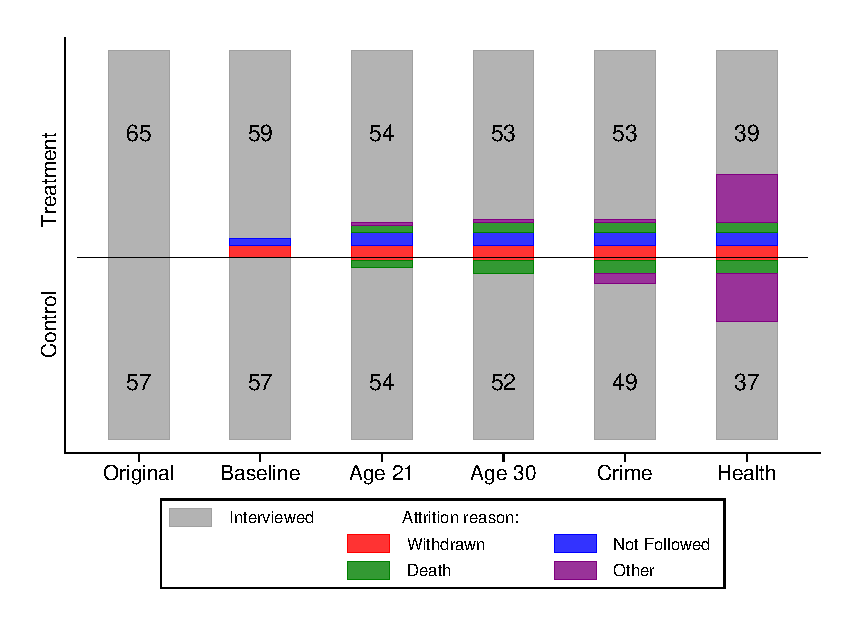
\includegraphics[height=2.5in]{output/abc_attrition.eps}
  \floatfoot{
\footnotesize
Note: This plot shows the number of participants, by experimental group, for whom there exists data at the periods of data collection. The children who were withdrawn from the study were done so due to several reasons including adoption. Children were not followed if they were found to be biologically retarded after randomization. The numbers in the bars indicate the number of individuals who were interviewed during that data collection. The original sample was measured after randomization but before the start of the program. The baseline sample was measured at the start of the program. The health sample was collected at age 34.
}
\end{figure}

\noindent For both programs, attrition is very low. In ABC, information is available on 100 children in the age 30 follow-up, which we call the adult follow-up. Figure~\ref{fig:abc-flow} describes the retention flow up to this follow-up. Additionally, 88 participants (45 and 43 from the control and treatment groups respectively) consented to release their criminal records and information on a full-range biomedical sweep is available (for 31 and 39 participants of the control and treatment groups, respectively). For example, the data indicate prevalence of diabetes and high blood pressure, waist-to-hip ratio, height and weight, and cholesterol levels. Table~\ref{tab:crime_baseline} and Table~\ref{tab:health_baseline} show the average balance in observed characteristics across the control and treatment groups at  baseline for individuals who released crime and health data.\\

\noindent \textbf{[JLG: tables comparing observables of crime and health respondents.]}

\section{Results}

\subsection{CARE}

\noindent \textbf{[JLG: Anna and Yu Kyung working in this subsection of CARE, as part of the objective of their April 2016 trip]}.

%References
\renewcommand{\refname}{Appendix References}
\clearpage
\singlespace
\bibliographystyle{chicago}
\bibliography{heckman}

\end{document} 